%%%%%%%% ICML 2025 EXAMPLE LATEX SUBMISSION FILE %%%%%%%%%%%%%%%%%

\documentclass{article}

% Recommended, but optional, packages for figures and better typesetting:
\usepackage{microtype}
\usepackage{graphicx}
\usepackage{subfigure}
\usepackage{booktabs} % for professional tables

% hyperref makes hyperlinks in the resulting PDF.
% If your build breaks (sometimes temporarily if a hyperlink spans a page)
% please comment out the following usepackage line and replace
% \usepackage{icml2025} with \usepackage[nohyperref]{icml2025} above.
\usepackage{hyperref}


% Attempt to make hyperref and algorithmic work together better:
\newcommand{\theHalgorithm}{\arabic{algorithm}}

% Use the following line for the initial blind version submitted for review:
\usepackage{icml2025}

% If accepted, instead use the following line for the camera-ready submission:
% \usepackage[accepted]{icml2025}

% For theorems and such
\usepackage{amsmath}
\usepackage{amssymb}
\usepackage{mathtools}
\usepackage{amsthm}

% if you use cleveref..
\usepackage[capitalize,noabbrev]{cleveref}

%%%%%%%%%%%%%%%%%%%%%%%%%%%%%%%%
% THEOREMS
%%%%%%%%%%%%%%%%%%%%%%%%%%%%%%%%
\theoremstyle{plain}
\newtheorem{theorem}{Theorem}[section]
\newtheorem{proposition}[theorem]{Proposition}
\newtheorem{lemma}[theorem]{Lemma}
\newtheorem{corollary}[theorem]{Corollary}
\theoremstyle{definition}
\newtheorem{definition}[theorem]{Definition}
\newtheorem{assumption}[theorem]{Assumption}
\theoremstyle{remark}
\newtheorem{remark}[theorem]{Remark}

% Todonotes is useful during development; simply uncomment the next line
%    and comment out the line below the next line to turn off comments
%\usepackage[disable,textsize=tiny]{todonotes}
\usepackage[textsize=tiny]{todonotes}


% The \icmltitle you define below is probably too long as a header.
% Therefore, a short form for the running title is supplied here:
\icmltitlerunning{Extraction of Experimental Variables from Scientific Papers}

\begin{document}

\twocolumn[
\icmltitle{Extraction of Experimental Variables from Scientific Papers}

% It is OKAY to include author information, even for blind
% submissions: the style file will automatically remove it for you
% unless you've provided the [accepted] option to the icml2025
% package.

% List of affiliations: The first argument should be a (short)
% identifier you will use later to specify author affiliations
% Academic affiliations should list Department, University, City, Region, Country
% Industry affiliations should list Company, City, Region, Country

% You can specify symbols, otherwise they are numbered in order.
% Ideally, you should not use this facility. Affiliations will be numbered
% in order of appearance and this is the preferred way.
\icmlsetsymbol{equal}{*}

\begin{icmlauthorlist}
\icmlauthor{GUERRIER Vanessa}{equal,yyy}
\icmlauthor{Firstname2 Lastname2}{equal,yyy,comp}
\icmlauthor{Firstname3 Lastname3}{comp}
\icmlauthor{Firstname4 Lastname4}{sch}
\icmlauthor{Firstname5 Lastname5}{yyy}
\icmlauthor{Firstname6 Lastname6}{sch,yyy,comp}
\icmlauthor{Firstname7 Lastname7}{comp}
%\icmlauthor{}{sch}
\icmlauthor{Firstname8 Lastname8}{sch}
\icmlauthor{Firstname8 Lastname8}{yyy,comp}
%\icmlauthor{}{sch}
%\icmlauthor{}{sch}
\end{icmlauthorlist}

\icmlaffiliation{yyy}{Master IAAA, Aix-Marseille University ,Marseille, France}
\icmlcorrespondingauthor{GUERRIER Vanessa}{vanessa.guerrier@etu.univ-amu.fr}
\icmlcorrespondingauthor{BELLILI Idir}{first2.last2@www.uk}

% You may provide any keywords that you
% find helpful for describing your paper; these are used to populate
% the "keywords" metadata in the PDF but will not be shown in the document
\icmlkeywords{Machine Learning}

\vskip 0.3in
]

% this must go after the closing bracket ] following \twocolumn[ ...

% This command actually creates the footnote in the first column
% listing the affiliations and the copyright notice.
% The command takes one argument, which is text to display at the start of the footnote.
% The \icmlEqualContribution command is standard text for equal contribution.
% Remove it (just {}) if you do not need this facility.

%\printAffiliationsAndNotice{}  % leave blank if no need to mention equal contribution
\printAffiliationsAndNotice{\icmlEqualContribution} % otherwise use the standard text.
\begin{abstract}
Recent advances in deep learning have increased interest in the environmental impact of machine learning models. Several studies aim to estimate carbon emissions using information reported in scientific publications.In this work, we propose an automatic approach to extract experimental variables from scientific articles based on Named Entity Recognition (NER). Our method uses BIO sequence tagging models trained on synthetically generated data and relies on BERT-based language representations to identify the key information required for carbon footprint estimation. Results show that, despite the structural heterogeneity of scientific papers, explicitly mentioned entities can be effectively extracted within a local context. Context window size significantly affects performance, highlighting a trade-off between precision and recall. Finally, synthetic data generation appears to be a relevant solution when annotated corpora are unavailable, provided sufficient diversity to ensure generalization.
\end{abstract}

\section{Introduction}

Nowadays, large-scale deep learning models achieve high performance. However, training these models requires a large amount of computational resources and energy. This energy consumption leads to $CO_{2}$ emissions. To estimate the carbon emissions produced during training, we need specific information, such as the hardware used, the training time, the country where the training was performed, and the year of training.

Most of this information is available in the scientific papers where the models are presented. Therefore, we need an automatic system to extract this information from scientific articles. The goal of our project is to develop a model based on BIO annotation to automatically extract these relevant data.

To train our models, we first created a training dataset. We then evaluated their performance on a generated test dataset using standard metrics such as precision, recall, and $F_{1}$-score, with a fuzzy matching approach. In addition, we evaluated the models on a real dataset, GreenMIR, using the same metrics as Thibaud and al. in their article \cite{greenwade93}.

So in Section 2, we describe how we generated the training dataset and introduce the GreenMIR dataset. In Section 3, we present the evaluation metrics and the models. In Section 4, we analyze and discuss the performance of the trained models. In Section 5, we estimate the carbon footprint of this project. Finally, in Section 6, we conclude and suggest directions for future work.

\section{Dataset}
This work relies on two distinct datasets. The first is a synthetically generated corpus, produced by prompting severl large language models (LLMs), and is used for training and intrinsic evaluation. The second is GreenMIR~\cite{holzapfel2024green}, a collection of real scientific papers from the ISMIR conference, which is used for extrinsic evaluation to assess the generalization capability of our models on real-world data.

\subsection{Synthetic Corpus Generation} 
Since no existing datset provides scientific articles annotated with the experimental variables we aim to extract, and since manual annotation is both time-consuming and costly, we opted for a synthetic data generation approach by prompting large language models. Each generated article simulates an excerpt from the experimental section of an AI research paper, where the seven target entities — model name, parameter count, GPU count, hardware type, training duration, country, and year — are annotated inline using XML tags (e.g., \texttt{<model>GPT-3</model>}).

The generation is guided by a carefully engineered prompt\footnote{Fullprompt available at:\url{https://github.com/Idir6380/TER_GENERATOR/blob/main/prompt.md}},designed following the advanced prompt engineering principles described in~\cite{alammar2024hands}. Specifically, our prompt covers six key components: a \textbf{persona} (an AI research expert), an \textbf{instruction} (generate a realistic experimental section excerpt), a \textbf{context} (the 7 entities to integrate naturally with temporal coherence constraints), a \textbf{format} (JSON output with inline XML tags), a \textbf{tone} (formal academic writing), and \textbf{five few-shot examples} covering different AI domains (NLP, Computer Vision, Speech, Reinforcement Learning, Bioinformatics).

To ensure diversity in writing style and thematic coverage, we used five different LLMs as generators: Claude Sonnet, Kimi, Qwen 3-32B, Gemini 2.5-flash, and Gemini 3-flash-preview. Fields are randomly omitted in each article, from zero to five per sample, to reflect the natural incompleteness of real scientific papers. The final corpus contains 478 articles after a cleaning step removing malformed generations. Table~\ref{tab:generation} summarizes the generation statistics for each LLM.

\begin{table}[H]
\centering
\resizebox{0.51\textwidth}{!}{
\begin{tabular}{|l|c|c|c|}
\hline
\textbf{Model} & \textbf{Articles} & \textbf{Avg. time/article (s)} & \textbf{Total time (min)} \\
\hline
Kimi                   & 99  & 5.3  & 8.6  \\
Claude Sonnet          & 100 & 11.0 & 18.1 \\
Gemini 2.5-flash       & 100 & 13.8 & 22.7 \\
Gemini 3-flash-preview & 88  & 42.6 & 61.7 \\
Qwen 3-32B             & 91  & 43.6 & 65.4 \\
\hline
\textbf{Total}         & \textbf{478} & \textbf{23.3} & \textbf{176.5} \\
\hline
\end{tabular}
}
\caption{Generation statistics per LLM.}
\label{tab:generation}
\end{table}

To verify the thematic diversity of the generated corpus, we applied topic modeling using BERTopic~\cite{grootendorst2022bertopic} framework. Nine coherent topics were identified, covering a wide range of AI research domains including NLP/LLMs, computer vision/Multimodal, speech \& audio, robotics, and bioinformatics, confirming that the corpus is not biased towards a single domain.

\subsection{GreenMIR Dataset}                                                 
GreenMIR~\cite{holzapfel2024green} is a collection of 113 real scientific papers from the ISMIR conference to study the environmental impact of music-AI research. For each paper, a ground truth table provides the values of the experimental variables of interest: hardware type, number of GPUs, training duration, number of parameters, country, and year. Since GreenMIR consists of real scientific papers, it is used exclusively as a \textbf{held-out test set} to evaluate the generalization of our models on real-world data.

\section{Model Architecture and Evaluation Metrics}

\subsection{Model and Architecture}

As mentioned previously, our objective was to build a model using BIO annotation to extract relevant information from scientific papers. After generating the training dataset, we annotated it using the labels presented in Table~\ref{tab:labels}.

\begin{table}[H]
\centering
\resizebox{0.51\textwidth}{!}{
\begin{tabular}{|l|c|}
\hline
\textbf{Label} & \textbf{Description} \\
\hline
B-gpu\_count & Number of GPUs used to train  \\
\hline
B-training & Beginning of the training duration \\
I-training & Inside the training duration  \\
\hline
B-model & Beginning of the model name\\
I-model & Inside the model name\\
\hline
B-hardware & Beginning of the hardware used\\
I-hardware & Inside the hardware \\
\hline
B-country & Beginning of the country where the model was trained \\
I-country & Inside the country \\
\hline
B-params & Beginning of the number of model parameters entity \\
I-params & Inside the number of model parameters entity \\
\hline
B-year & Beginning of the training year entity \\
\hline
O & Tokens outside any entity \\
\hline
\end{tabular}
}
\caption{Labels used for annotation}
\label{tab:labels}
\end{table}

For experimentation, we selected several models for training, as: DistilBERT and  SciBERT which are presented below. The Annex section contains a table (Table~\ref{tab:training_config}) reporting the configuration of each model used.

\subsubsection{DistilBERT}
We used this model as an initial experiment to evaluate its behavior when trained on generated data. For this purpose, we adopted the \texttt{AutoModelForTokenClassification} architecture along with its corresponding tokenizer.We experimented with two different approaches. In the first approach, DistilBERT\cite{sanh2019distilbert} generates a contextual representation vector based on the input sentence; therefore, each input consists of a single sentence. In the second approach, we used the same architecture, but with an additional contextual sentence provided alongside the main sentence. In this setting, each input is composed of the target sentence and an additional sentence serving as context.Each approach contains more than 65M parameters, of which only 11k are trainable. Both versions of the model were trained twice. In the first approach, each run took approximately 3 hours, while in the second approach, each run took about 7 hours. Therefore, the models were trained for a total of approximately 20 hours.
%\subsubsection{Google-BERT}
%After evaluating the performance of DistilBERT\cite{sanh2019distilbert}, we experimented with a larger pretrained BERT\cite{devlin2019bert} model. For this model, we adopted the \texttt{AutoModel} architecture along with its corresponding tokenizer and applied a full fine-tuning strategy. We implemented a custom token classification head composed of a dropout layer followed by a linear layer. The last hidden state of BERT is used as the contextual feature representation for each token. The inputs to the model consist of tokenized sentences, and the parameters of the classification layer are updated during training.

\subsubsection{SciBERT with Layer-wise Fine-tuning}
We selected SciBERT~\cite{DBLP:journals/corr/abs-1903-10676} as our base model, a BERT-base variant pretrained on 1.14 million scientific papers, making it particularly suited to our domain-specific extraction task. Following~\cite{jawahar2019bert}, we adopt a layer-wise fine-tuning strategy where only the last $k \in \{0, 1, 2, 4\}$ encoder layers are unfrozen. Token representations are extracted from four candidate layers (L8, L10, L12, AVG)~\cite{devlin2019bert}, and a sliding window of size $c \in \{0, 1, 2\}$~\cite{luoma2020crosssentence} provides cross-sentence context. A dropout layer (0.1) and a linear projection head map the selected representations to the BIO label space. To ensure coherence between the fine-tuning depth and the extraction layer, configurations where the number of unfrozen layers exceeds the index of the extraction layer are discarded, reducing the grid from $4 \times 4 \times 3 = 48$ to \textbf{39 valid configurations}.

The full grid search was conducted on an NVIDIA RTX 3090 (24 GB) via Vast.ai, with early stopping (patience = 5). The best configuration (\textbf{F4\_AVG\_2}) alone required approximately 7 minutes, while the complete grid search totaled approximately 2 hours.

A key design choice concerns the data splitting strategy. An initial sentence-level split — where individual sentences are randomly assigned to train, validation, and test sets — introduces \textbf{data leakage}: sentences from the same article can appear in both the training and test sets, and the sliding window further increases overlap between splits. To address this, we adopt an \textbf{article-level split} (80/10/10), where all sentences of a given article belong exclusively to one split. This yields a more realistic evaluation, as confirmed by the lower but more reliable F1 scores obtained under this setting.

\subsection{Evaluation Metrics} 
We adopt the two-level evaluation framework proposed by Schneeberger~\cite{greenwade93}, which distinguishes between the \emph{presence} of a prediction and the \emph{quality} of its value.\\


\textbf{Categorical Metrics}: evaluate the correctness of extracted values for each field based on a direct comparison with the ground truth. Three cases are distinguished:

\begin{itemize}
    \item \textbf{True Positive (TP):} value correctly detected and matching the reference
    \item \textbf{False Positive (FP):} value detected but absent from the ground truth
    \item \textbf{False Negative (FN):} value present in the ground truth but not extracted
\end{itemize}

Based on these quantities, standard indicators are computed:

\begin{itemize}
    \item \textbf{Precision:} proportion of detected values that are correct
    \item \textbf{Recall:} proportion of reference values that are correctly retrieved
    \item \textbf{F1 Score:} harmonic mean of precision and recall
\end{itemize}
These metrics rely on a binary evaluation of correspondence.\\

\textbf{Distance Metrics }:aim to evaluate the quality of extracted values beyond their mere presence. For each field, a similarity score is defined as:
\[
S = 1 - d
\]
where \( d \) represents a distance measuring the difference between the extracted value and the reference value according to a metric adapted to the field type. The smaller the distance, the higher the similarity.
So-called \textit{soft} metrics are then computed:
\begin{itemize}
    \item Aligned Precision($P_{a}$): average similarity score computed over true positives only; it measures the quality of correct matches.
    \item Global Precision ($P_{g}$): average similarity score computed over all detected values (true positives and false positives); it penalizes hallucinations by counting them as complete errors in the denominator.
    \item Soft Recall($R_{s}$): average similarity score computed over the total number of expected values (true positives and false negatives); it measures the quality of reference information retrieval.
    \item Global Soft F1 Score($F1_{s}$): harmonic mean of global precision and soft recall, providing a synthetic performance measure that accounts for both accuracy and completeness of extracted values.
\end{itemize}

\section{Model Evaluation}

In this section, we present the performance of each model on the generated test set and then on the GreenMIR dataset.

\subsection{Evaluation on the Generated Dataset}

After training our models, we evaluated their performance on the generated test dataset. The results obtained are presented below.
\subsubsection{\textbf{Performance of DistilBERT Models}}

In the figures below:Fig\ref{fig:distilbert_loss1} and Fig\ref{fig:distilbert_loss2}, we present the evolution of the loss during training on the generated dataset. We observe that for both models, after approximately seven epochs, the loss starts to increase rather than decrease. This behavior continues intermittently until the last epoch. This pattern may indicate that both models begin to overfit after the seventh epoch.
\begin{figure}[H]
    \centering
    \includegraphics[width=0.70\linewidth]{Capture d’écran 2026-03-05 à 16.13.00.png}
    \caption{Training loss evolution of the first DistilBERT model without context.}
    \label{fig:distilbert_loss1}
\end{figure}

\begin{figure}[H]
    \centering
    \includegraphics[width=0.70\linewidth]{Capture d’écran 2026-03-05 à 16.13.35.png}
    \caption{Training loss evolution of the second DistilBERT model with context.}
    \label{fig:distilbert_loss2}
\end{figure}
After evaluating the models on the generated test set and the evaluation set, we used precision, recall and $F_{1}$-score as evaluation metrics, based on a fuzzy matching approach. This fuzzy approach ensures that tokens labeled as ''O'' are ignored during the evaluation, and only the entities are considered. Also, the fuzzy matching prevents penalizing the model when only part of an entity is correctly predicted.

\begin{table}[H]
\centering
\begin{tabular}{lccc}
\hline
Dataset & Precision & Recall & F1-score \\
\hline
\multicolumn{4}{l}{\textbf{Performance of the model without context}} \\
\hline
Test  & 0.88 & \textbf{0.95} & 0.92 \\
Evaluation  & 0.90 & \textbf{0.95} & 0.93 \\
\hline
\multicolumn{4}{l}{\textbf{Performance of the model with context}} \\
\hline
Test & 0.86 & \textbf{0.97} & 0.91 \\
Evaluation & 0.89 & \textbf{0.97} & 0.93 \\
\hline
\end{tabular}
\caption{Performance metrics on the test set and the evaluation set.}
\label{tab:results}
\end{table}
As shown in Table~\ref{tab:results}, both models achieve strong performance on the test and evaluation datasets. The model trained without contextual information achieves higher precision, indicating fewer false positives. In contrast, the model trained with contextual information obtains higher recall, suggesting that it is able to detect more entities overall. This improvement in recall may be explained by the additional contextual information provided during training, which helps the model better identify entities within the text. However, this also decreases precision, indicating that the model may produce more false positives when using context.

\subsubsection{\textbf{Performance of SciBERT Models}}

Among the 39 valid configurations trained with the article-level split, the top 3 models — all using the AVG layer extraction with full fine-tuning (F4) — are reported in Table~\ref{tab:scibert_top3}. The best configuration is \textbf{F4\_AVG\_2} (4 unfrozen layers, AVG of last 4 layers, context window of 2).

\begin{table}[H]
\centering
\resizebox{0.51\textwidth}{!}{
\begin{tabular}{|l|c|c|c|c|c|}
\hline
\textbf{Config} & \textbf{Finetune} & \textbf{Layer} & \textbf{Context} & \textbf{Eval F1} & \textbf{Test F1} \\
\hline
\rowcolor{yellow!30}
\textbf{F4\_AVG\_2} & \textbf{F4} & \textbf{AVG} & \textbf{2} & \textbf{0.9637} & \textbf{0.9610} \\
F4\_AVG\_0 & F4 & AVG & 0 & 0.9635 & 0.9640 \\
F4\_AVG\_1 & F4 & AVG & 1 & 0.9635 & 0.9632 \\
\hline
\end{tabular}
}
\caption{Top 3 SciBERT configurations (article-level split). Test F1 refers to macro F1.}
\label{tab:scibert_top3}
\end{table}

\subsection{Evaluation on GreenMIR Dataset}
To assess the generalization capability of our models on real-world data, we evaluate the best SciBERT configuration, \textbf{F4\_AVG\_2} and both of the approche using DistilBERT as model, on the GreenMIR dataset using the two-level evaluation framework described in Section~\ref{sec:metrics}. Table~\ref{tab:greenmir_best} reports the per-field results.

\begin{table}[H]
\centering
\resizebox{0.48\textwidth}{!}{
\begin{tabular}{|l|c|c|c|c|c|c|}
\hline
\textbf{Field} & \textbf{TP} & \textbf{FP} & \textbf{FN} & \textbf{P} & \textbf{R} & \textbf{F1} \\
\hline
year               & 65 & 0  & 48 & 1.00 & 0.57 & 0.73 \\
gpu\_count         & 16 & 4  & 14 & 0.80 & 0.53 & 0.64 \\
training\_duration &  9 & 10 & 17 & 0.47 & 0.34 & 0.40 \\
parameter\_count   &  3 & 15 & 10 & 0.16 & 0.23 & 0.19 \\
country            & 17 & 13 & 63 & 0.56 & 0.21 & 0.30 \\
hardware           & 30 &  5 & 13 & 0.85 & 0.69 & \textbf{0.76} \\
model\_name        & 43 &  0 & 70 & 1.00 & 0.38 & 0.55 \\
\hline
\textbf{macro avg} &    &    &    & \textbf{0.69} & \textbf{0.42} & \textbf{0.51} \\
\hline
\end{tabular}
}
\caption{Categorical metrics of F4\_AVG\_2 on GreenMIR.}
\label{tab:greenmir_cat}
\end{table}

\begin{table}[H]
\centering
\resizebox{0.48\textwidth}{!}{
\begin{tabular}{|l|c|c|c|c|c|c|}
\hline
\textbf{Field} & \textbf{TP} & \textbf{FP} & \textbf{FN} & \textbf{P} & \textbf{R} & \textbf{F1} \\
\hline
year                 & 80 & 0 & 33 & 1.00 & 0.71 & 0.83 \\
gpu\_count           & 7 & 0 & 23 & 1.00 & 0.23 & 0.38 \\
training\_duration   & 6 & 6 & 20 & 0.50 & 0.23 & 0.32 \\
parameter\_count     & 2 & 9 & 11 & 0.18 & 0.15 & 0.17 \\
country              & 29 & 9 & 51 & 0.76 & 0.36 & 0.49 \\
hardware             & 13 & 1 & 30 & 0.93 & 0.30 & 0.46 \\
model\_name          & 100 & 0 & 13 & 1.00 & 0.89 & \textbf{0.94} \\
\hline
\textbf{macro avg} & & & & \textbf{0.77} & \textbf{0.41} &\textbf{ 0.51} \\
\hline
\end{tabular}
}
\caption{Categorical metrics of DistilBERT model without context}
\end{table}


\begin{table}[H]
\centering
\resizebox{0.48\textwidth}{!}{
\begin{tabular}{|l|c|c|c|c|c|c|}
\hline
\textbf{Field} & \textbf{TP} & \textbf{FP} & \textbf{FN} & \textbf{P} & \textbf{R} & \textbf{F1} \\
\hline
year                     & 81 & 0 & 32 & 1.00 & 0.72 & 0.84 \\
gpu\_count               & 7 & 0 & 23 & 1.00 & 0.23 & 0.38 \\
training\_duration       & 7 & 6 & 19 & 0.54 & 0.27 & 0.36 \\
parameter\_count         & 2 & 20 & 11 & 0.09 & 0.15 & 0.11 \\
country                  & 29 & 13 & 51 & 0.69 & 0.36 & 0.48 \\
hardware                 & 17 & 1 & 26 & 0.94 & 0.40 & 0.56 \\
model\_name              & 112 & 0 & 1 & 1.00 & 0.99 & \textbf{1.00} \\
\hline
\textbf{macro avg} & & & & \textbf{0.75} & \textbf{0.45} & \textbf{0.53} \\
\hline
\end{tabular}
}
\caption{Categorical metrics of DistilBERT model with context}
\end{table}

\begin{table}[H]
\centering
\resizebox{0.48\textwidth}{!}{
\begin{tabular}{|l|c|c|c|c|}
\hline
\textbf{Field} & \textbf{$P_a$} & \textbf{$P_g$} & \textbf{$R_s$} & \textbf{$F1_s$} \\
\hline
year               & 0.99 & 0.99 & 0.57 & \textbf{0.72} \\
gpu\_count         & 0.85 & 0.68 & 0.45 & 0.55 \\
training\_duration & 0.68 & 0.32 & 0.23 & 0.27 \\
parameter\_count   & 0.33 & 0.05 & 0.07 & 0.06 \\
country            & 0.23 & 0.13 & 0.05 & 0.07 \\
hardware           & 0.73 & 0.62 & 0.51 & 0.56 \\
model\_name        & 0.41 & 0.41 & 0.15 & 0.22 \\
\hline
\textbf{macro avg} & \textbf{0.60} & \textbf{0.46} & \textbf{0.29} & \textbf{0.35} \\
\hline
\end{tabular}
}
\caption{Soft metrics of F4\_AVG\_2 on GreenMIR.}
\label{tab:greenmir_soft}
\end{table}

\begin{table}[H]
\centering
\resizebox{0.48\textwidth}{!}{
\begin{tabular}{|l|c|c|c|c|}
\hline
\textbf{Field} & \textbf{$P_a$} & \textbf{$P_g$} & \textbf{$R_s$} & \textbf{$F1_s$} \\
\hline
year                        & 0.99 & 0.99 & 0.70 & \textbf{0.82}  \\
gpu\_count                  & 1.00 & 1.00 & 0.23 & 0.38  \\
training\_duration          & 0.36 & 0.18 & 0.08 & 0.11  \\
parameter\_count            & 0.00 & 0.00 & 0.00 & 0.00  \\
country                     & 0.10 & 0.08 & 0.04 & 0.05  \\
hardware                    & 1.00 & 0.93 & 0.30 & 0.46  \\
model\_name                 & 0.31 & 0.31 & 0.27 & 0.29 \\
\hline
\textbf{macro avg} & \textbf{0.54} & \textbf{0.50} & \textbf{0.23} & \textbf{0.30} \\
\hline
\end{tabular}
}
\caption{Soft metrics of DistilBERT without context on GreenMIR.}
\end{table}


\begin{table}[H]
\centering
\resizebox{0.48\textwidth}{!}{
\begin{tabular}{|l|c|c|c|c|}
\hline
\textbf{Field} & \textbf{$P_a$} & \textbf{$P_g$} & \textbf{$R_s$} & \textbf{$F1_s$} \\
\hline
year                      & 0.99 & 0.99 & 0.71 & \textbf{0.83} \\
gpu\_count                & 0.89 & 0.89 & 0.21 & 0.34 \\
training\_duration        & 0.46 & 0.25 & 0.12 & 0.17 \\
parameter\_count          & 0.00 & 0.00 & 0.00 & 0.00 \\
country                   & 0.10 & 0.07 & 0.04 & 0.05 \\
hardware                  & 0.88 & 0.83 & 0.35 & 0.49 \\
model\_name               & 0.35 & 0.35 & 0.35 & 0.35 \\
\hline
\textbf{macro avg} & \textbf{0.53} & \textbf{0.48} & \textbf{0.25} & \textbf{0.32} \\
\hline
\end{tabular}
}
\caption{Soft metrics of DistilBERT with context on GreenMIR.}
\end{table}

The tree models achieve perfect categorical precision on \texttt{year} and \texttt{model\_name}, with no false positives. They also obtain the best F1 score on \texttt{hardware} with F4\_AVG\_2. In the other settings, \texttt{model\_name} consistently shows the highest F1 score, making it the easiest field to detect. DistilBERT models also show very high precision on \texttt{year}, \texttt{gpu\_count}, and \texttt{model\_name}, often close to perfect. However, \texttt{gpu\_count} has low recall: predictions are usually correct, but many true cases are missed. This suggests difficulty with numerical or rarely mentioned information.Overall, recall is the main weakness across models, especially for \texttt{country}, \texttt{training\_duration}, and \texttt{parameter\_count}, which are harder to detect due to implicit mentions and varied formats.

The soft precision metric $P_a$ confirms that extracted values are accurate when detected. For example, \texttt{year} reaches an aligned precision of 0.99 for all models, showing that dates are easy to extract correctly. In contrast, numerical fields such as \texttt{parameter\_count} and \texttt{training\_duration} obtain very low soft scores, indicating difficulties in precise value extraction.
Overall, DistilBERT with context offers the best balance between precision and recall, while the tree models remain strong for accurate extraction in structured fields.


%The soft precision $P_a$ confirms the quality of extracted values when the model does predict: 0.99 for \texttt{year} for all the models and 0.859 for \texttt{gpu\_count}. The weakest field is \texttt{parameter\_count} ($F1_s$=0.065), where the model frequently confuses sequence lengths, GPU memory sizes, and dataset sizes with actual parameter counts. The recall on \texttt{country} is improved by a city-to-country normalization step (e.g., \textit{Milan} $\rightarrow$ \textit{Italy}), which increased the true positives from 4 to 17.


\section{Carbon Footprint Estimation}
After training and evaluating different models, we want to assess the carbon footprint of this project. To do so, we use the formula below, which allows us to calculate the carbon intensity (gCO$_2$/kWh) per model:
\[CO_2 = N_{gpu} \times P_{gpu} \times T_{training} \times C_I \times 10^{-3}\]

{\small where $N_{gpu}$ = number of GPUs, $P_{gpu}$ = power draw (W),
$T_{training}$ = training duration (h), $C_I$ = carbon intensity (gCO$_2$/kWh)}.

The SciBERT grid search was conducted on a single NVIDIA RTX 3090 ($P_{gpu} = 350$\,W, $N_{gpu} = 1$) via Vast.ai, hosted in the Czech Republic ($C_I = 400$\,gCO$_2$/kWh, IEA 2022). The DistilBERT models were trained on a personal laptop equipped with a 8 GB of 1600 MHz DDR3 RAM and Intel Core i5 dual-core at 1.8\,GHz ($P_{cpu} = 15$\,W), located in France ($C_I = 52$\,gCO$_2$/kWh, IEA 2022). For CPU-based training, Equation~\ref{eq:co2} is applied with $P_{gpu}$ replaced by $P_{cpu}$.

\begin{table}[H]
\centering
\small
\begin{tabular}{|l|c|c|c|c|}
\hline
\textbf{Model} & \textbf{Hardware} & \textbf{$T_{training}$} & \textbf{$C_I$} & \textbf{CO$_2$ (g)} \\
\hline
SciBERT (full grid)  & RTX 3090, 350\,W & 2\,h    & 400 & 280.0 \\
SciBERT (best only)  & RTX 3090, 350\,W & 7\,min  & 400 &  16.4 \\
\hline
DistilBERT 1 (×2)    & i5 CPU, 15\,W    & 6\,h    &  52 &   4.7 \\
DistilBERT 2 (×2)    & i5 CPU, 15\,W    & 14\,h   &  52 &  10.9 \\
\hline
\end{tabular}
\caption{\small Estimated CO$_2$ emissions per model. SciBERT trained in Czech Republic; DistilBERT trained in France.}
\label{tab:co2}
\end{table}

SciBERT's full grid search emits 280\,gCO$_2$ (equivalent to roughly 1.3\,km driven by car), while training the best configuration alone costs only 16\,gCO$_2$. DistilBERT training on CPU in France produces far less — between 4.7 and 10.9\,gCO$_2$ — owing to both the lower hardware power draw and the cleaner French electricity grid. These figures illustrate how carbon cost depends heavily on hardware choice and data center location, and motivate the use of systematic variable extraction to enable such estimates at scale.

\section{Discussion \& Conclusion}

This work demonstrates the feasibility of automated extraction of experimental variables from scientific publications using BIO-based sequence tagging models trained on synthetically generated data. Despite the structural heterogeneity of real scientific papers, models operating on small contextual windows successfully extracted relevant entities when explicitly mentioned in a local context, as evidenced by near-perfect precision on \texttt{year} and \texttt{model\_name} across all configurations. The contextual window size significantly influences extraction performance: DistilBERT with context achieves higher recall at the cost of precision, while SciBERT F4\_AVG\_2 offers the best overall balance. However, recall remains the primary limitation across all models, particularly for \texttt{country}, \texttt{training\_duration}, and \texttt{parameter\_count}, whose implicit mentions and heterogeneous formats pose persistent challenges. Furthermore, synthetic data generation via LLMs proves to be a viable strategy in the absence of annotated corpora, though domain coverage and structural diversity remain critical factors for generalization to real-world data.

Building on these findings, several directions are envisioned for future work. First, extending synthetic generation to full articles rather than experimental sections only would better reflect the structural complexity of real publications. Second, adopting longer-context architectures such as Longformer (4096 tokens) would enable the capture of entities distributed across full documents without truncation. Finally, \textbf{towards a standardized reporting taxonomy}: authors of scientific publications should adhere to a structured reporting convention that systematically documents all variables necessary for carbon impact computation — including hardware specifications, training duration, and geographic location — within a dedicated section, so as to enable automated extraction at reduced computational cost.



\nocite{langley00}

\bibliography{example_paper}
\bibliographystyle{icml2025}


%%%%%%%%%%%%%%%%%%%%%%%%%%%%%%%%%%%%%%%%%%%%%%%%%%%%%%%%%%%%%%%%%%%%%%%%%%%%%%%
%%%%%%%%%%%%%%%%%%%%%%%%%%%%%%%%%%%%%%%%%%%%%%%%%%%%%%%%%%%%%%%%%%%%%%%%%%%%%%%
% APPENDIX
%%%%%%%%%%%%%%%%%%%%%%%%%%%%%%%%%%%%%%%%%%%%%%%%%%%%%%%%%%%%%%%%%%%%%%%%%%%%%%%
%%%%%%%%%%%%%%%%%%%%%%%%%%%%%%%%%%%%%%%%%%%%%%%%%%%%%%%%%%%%%%%%%%%%%%%%%%%%%%%
\newpage
\appendix
\onecolumn


\section{Corpus Analysis}

\begin{figure}[H]
    \centering
    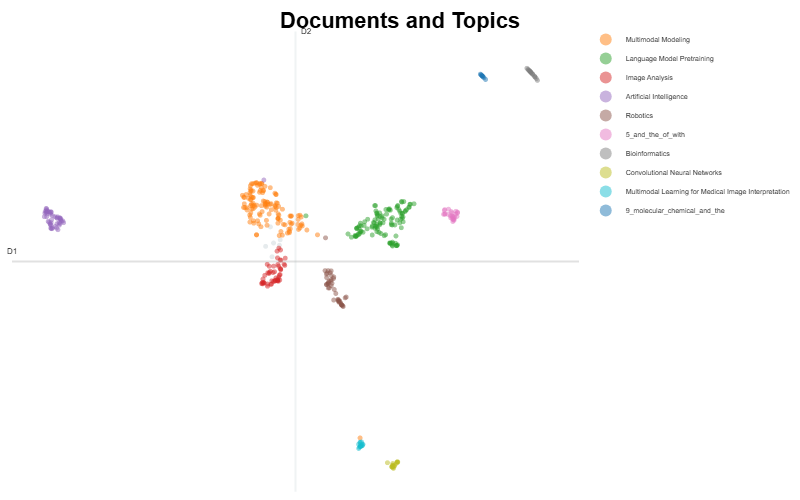
\includegraphics[width=0.8\linewidth]{plots/topics.png}
    \caption{\small Nine topics identified by BERTopic on the 478-article synthetic corpus.}
    \label{fig:topics}
\end{figure}

\begin{figure}[H]
    \centering
    \includegraphics[width=0.7\linewidth]{plots/global_top10_hardware_countries_years.png}
    \caption{\small Top-10 hardware types, countries, and years across the synthetic corpus.}
    \label{fig:top10}
\end{figure}

\begin{figure}[H]
    \centering
    \includegraphics[width=0.7\linewidth]{plots/global_omission_analysis.png}
    \caption{\small Field omission distribution per LLM generator.}
    \label{fig:omissions}
\end{figure}

\begin{figure}[H]
    \centering
    \includegraphics[width=0.7\linewidth]{plots/global_xml_tag_compliance.png}
    \caption{\small XML tag compliance rate per LLM generator.}
    \label{fig:compliance}
\end{figure}

\section{SciBERT Training Curves}

\begin{figure}[H]
    \centering
    \begin{minipage}{0.48\linewidth}
        \centering
        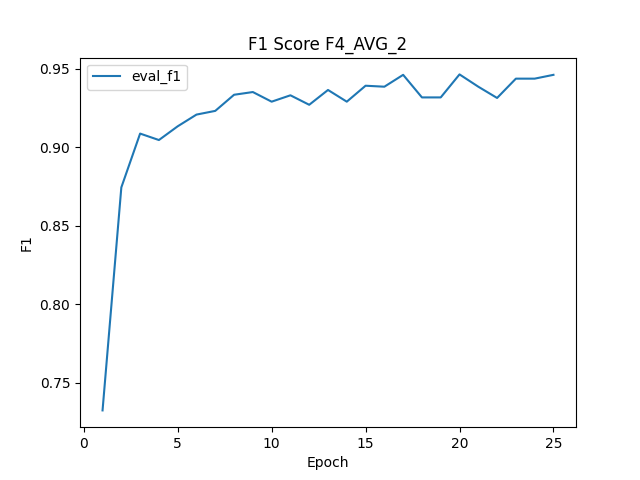
\includegraphics[width=\linewidth]{plots/best_model_f1_scibert_curves.png}
        \caption{\small F1 evolution during training of the best SciBERT configuration (F4\_AVG\_2).}
    \end{minipage}
    \hfill
    \begin{minipage}{0.48\linewidth}
        \centering
        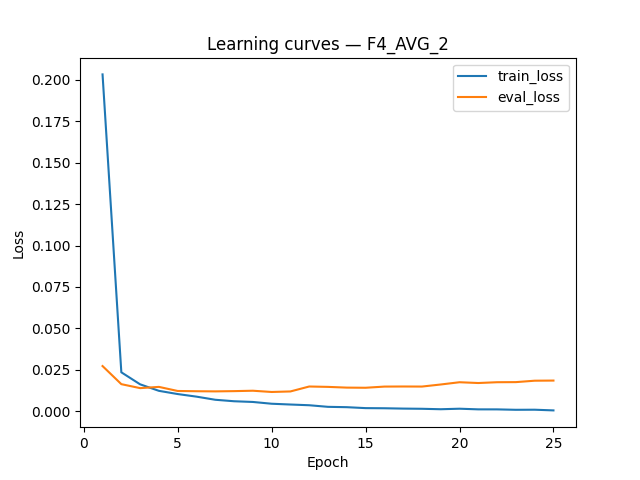
\includegraphics[width=\linewidth]{plots/best_model_loss_scibert_curves.png}
        \caption{\small Loss evolution during training of the best SciBERT configuration (F4\_AVG\_2).}
    \end{minipage}
\end{figure}
\section{Training Configuration}

\begin{table}[H]
\centering
\small
\begin{tabular}{|l|c|c|c|c|c|}
\hline
Model & Padding & Parameters & Batch & Epochs & Time \\
\hline
DistilBERT 1 & 200 & 11K / \textbf{65M} & 32 & 10 & $2 \times 3$ h \\
\hline
DistilBERT 2 & 400 & 11K / \textbf{65M} & 32 & 10 & $2 \times 7$ h \\
\hline
SciBERT & 512 & 11K / \textbf{109M} & 64 & 300 & $\sim$2h \\
\hline
\end{tabular}
\caption{\small Training configuration of the evaluated models. Time: total training time. Padding: maximum padding length. Parameters: trainable / total (bold). Batch: batch size. Epochs: total training epochs.}
\label{tab:training_config}
\end{table}
%%%%%%%%%%%%%%%%%%%%%%%%%%%%%%%%%%%%%%%%%%%%%%%%%%%%%%%%%%%%%%%%%%%%%%%%%%%%%%%
%%%%%%%%%%%%%%%%%%%%%%%%%%%%%%%%%%%%%%%%%%%%%%%%%%%%%%%%%%%%%%%%%%%%%%%%%%%%%%%


\end{document}


% This document was modified from the file originally made available by
% Pat Langley and Andrea Danyluk for ICML-2K. This version was created
% by Iain Murray in 2018, and modified by Alexandre Bouchard in
% 2019 and 2021 and by Csaba Szepesvari, Gang Niu and Sivan Sabato in 2022.
% Modified again in 2023 and 2024 by Sivan Sabato and Jonathan Scarlett.
% Previous contributors include Dan Roy, Lise Getoor and Tobias
% Scheffer, which was slightly modified from the 2010 version by
% Thorsten Joachims & Johannes Fuernkranz, slightly modified from the
% 2009 version by Kiri Wagstaff and Sam Roweis's 2008 version, which is
% slightly modified from Prasad Tadepalli's 2007 version which is a
% lightly changed version of the previous year's version by Andrew
% Moore, which was in turn edited from those of Kristian Kersting and
% Codrina Lauth. Alex Smola contributed to the algorithmic style files.
